\documentclass[a4paper, 12pt]{article}

\usepackage[utf8]{inputenc}
\usepackage[T5]{fontenc}
\usepackage[vietnamese]{babel}

\usepackage[a4paper,margin=24mm]{geometry}
\usepackage[skip=10pt plus1pt, indent=20pt]{parskip}
\usepackage{indentfirst}
\usepackage{fancyhdr}
\usepackage{titlesec}
\usepackage{tocbasic}

\usepackage{amsmath,amssymb}
\usepackage{textcomp}
\usepackage{gensymb}

\usepackage{graphicx}
\usepackage{subfig}
\usepackage{subcaption}
\usepackage{xcolor}

\usepackage[colorlinks=true,allcolors=blue,urlcolor=magenta]{hyperref}

\usepackage{minted}
\usepackage{listings}
\usepackage{verbatim}

\usepackage{relsize}
\usepackage{array}

\usepackage[colorinlistoftodos]{todonotes}

\usepackage{lipsum}
\usepackage[normalem]{ulem}
\usepackage{xparse}

\NewDocumentCommand{\myrule}{O{1pt} O{2pt} O{black}}{%
  \par\nobreak%
  \kern\the\prevdepth%
  \kern#2
  {\color{#3}\hrule height #1 width\hsize} 
  \kern#2
  \nointerlineskip%
}

\usepackage[section]{placeins}

\usepackage{booktabs}    
\usepackage{colortbl}   
\newcommand{\myrowcolour}{\rowcolor[gray]{0.925}} 

\DeclareTOCStyleEntry[
  indent=12pt,
  level=1
]{largetocline}{section}

\setlength{\marginparwidth}{2cm}

\begin{document}
\thispagestyle{empty}
\begin{titlepage}
  \begin{center}
    \textbf{\LARGE ĐẠI HỌC QUỐC GIA}\\
    \textbf{\LARGE THÀNH PHỐ HỒ CHÍ MINH}\\[0.5cm]
    \vspace{20pt}
    \textbf{\large TRƯỜNG ĐẠI HỌC KHOA HỌC TỰ NHIÊN}\\[0.2cm]
    \textbf{\large KHOA CÔNG NGHỆ THÔNG TIN}\\[0.2cm]
    \vspace{20pt}
    
\includegraphics[width=0.4\textwidth,keepaspectratio]{imgs/logo.png}

    \par
    \vspace{20pt}
    \textbf{\Large MTH00057 - Toán ứng dụng và thống kê cho Công nghệ thông tin}\\
    \vspace{15pt}
    \myrule[1pt][7pt]
    \textbf{\LARGE BÁO CÁO ĐỒ ÁN 2}\\
    \vspace{15pt}
    \textbf{\Large Image Processing}\\
    \vspace{10pt}
    \myrule[1pt][7pt]
    \vspace{25pt}

    \begin{tabular}{c@{\hspace{2cm}}c}
      \textbf{Họ tên} & \textbf{MSSV} \\
      Bùi Minh Duy    & 23127040      \\
    \end{tabular}

    \vspace{10pt}
    \textbf {Giảng viên hướng dẫn}\\[0.2cm]
    Nguyễn Văn Quang Huy \\ Trần Hà Sơn \\ Nguyễn Đình Thúc\\ Nguyễn Ngọc Toàn

    \vspace{25pt}
    \today

  \end{center}
\end{titlepage}

\newpage

\tableofcontents\thispagestyle{empty}
\newpage

\section{Thông tin cá nhân}

\begin{itemize}
	\item Họ và tên: Bùi Minh Duy
	\item MSSV: 23127040
	\item Lớp: 23CLC01
\end{itemize}

\section{Các chức năng đã hoàn thành}

\begin{table}[H]
	\centering
	\renewcommand{\arraystretch}{1.3}
	\begin{tabular}{|p{8cm}|>{\centering\arraybackslash}p{5cm}|}
		\hline
		\textbf{Chức năng}                       & \textbf{Mức độ hoàn thành} \\
		\hline
		Điều chỉnh độ sáng của ảnh               & 100\%                      \\
		\hline
		Điều chỉnh độ tương phản của ảnh         & 100\%                      \\
		\hline
		Chuyển ảnh RGB sang màu xám (grayscale)  & 100\%                      \\
		\hline
		Chuyển ảnh RGB sang màu sepia            & 100\%                      \\
		\hline
		Làm mờ ảnh                               & 100\%                      \\
		\hline
		Làm nét ảnh                              & 100\%                      \\
		\hline
		Lật ảnh theo chiều ngang và dọc          & 100\%                      \\
		\hline
		Cắt ảnh theo khung hình vuông            & 100\%                      \\
		\hline
		Cắt ảnh theo khung hình tròn             & 100\%                      \\
		\hline
		Cắt ảnh theo khung 2 hình elip chéo nhau & 100\%                      \\
		\hline
	\end{tabular}
	\caption{Danh sách các chức năng và mức độ hoàn thành}
\end{table}

\newpage
\section{Ý tưởng thực hiện và mô tả các hàm chức năng}

\subsection{Điều chỉnh độ sáng (Hàm \texttt{adjust\_brightness})}

\subsubsection*{Ý tưởng thực hiện}

Hàm \texttt{adjust\_brightness} điều chỉnh độ sáng của ảnh bằng cách cộng trực tiếp một giá trị độ sáng (\texttt{value}) vào từng điểm ảnh. Đây là một cách điều chỉnh tuyến tính đơn giản nhưng hiệu quả để làm thay đổi độ sáng tổng thể của ảnh.
\begin{itemize}
  \item Nếu \texttt{value > 0}, ảnh sẽ sáng hơn.
  \item Nếu \texttt{value < 0}, ảnh sẽ tối đi.
  \item Nếu \texttt{value = 0}, ảnh giữ nguyên độ sáng.
\end{itemize}

\subsubsection*{Mô tả chi tiết}

Hàm nhận vào ảnh RGB đầu vào dưới dạng NumPy array và một giá trị số thực \texttt{value} đại diện cho mức độ điều chỉnh độ sáng.

Đầu tiên, ảnh được ép kiểu sang \texttt{float32} để đảm bảo phép cộng được thực hiện chính xác mà không bị tràn số. Sau đó, giá trị độ sáng được cộng trực tiếp vào từng phần tử (tức là từng kênh màu tại mỗi điểm ảnh) trong ảnh.

Kết quả thu được có thể chứa các giá trị vượt ngoài khoảng [0, 255], nên cần dùng hàm \texttt{clip} để giới hạn toàn bộ ảnh về trong khoảng hợp lệ này.

Cuối cùng, ảnh được chuyển ngược lại về kiểu \texttt{uint8} để sẵn sàng hiển thị hoặc lưu trữ.

\subsection{Điều chỉnh độ tương phản (Hàm \texttt{adjust\_contrast})}

\subsubsection*{Ý tưởng thực hiện}

Hàm \texttt{adjust\_contrast} cho phép điều chỉnh độ tương phản của một ảnh RGB bằng cách làm giãn hoặc co khoảng cách giữa các mức cường độ sáng so với mức sáng trung bình thực tế của ảnh. Việc thay đổi độ tương phản được điều khiển bằng hệ số \texttt{alpha}:
\begin{itemize}
  \item Nếu \texttt{alpha > 1}, độ tương phản tăng: điểm ảnh sáng trở nên sáng hơn, điểm tối trở nên tối hơn.
  \item Nếu \texttt{0 < alpha < 1}, độ tương phản giảm: ảnh trở nên mờ nhạt hơn.
  \item Nếu \texttt{alpha = 1}, ảnh giữ nguyên.
\end{itemize}

\subsubsection*{Mô tả chi tiết}

Hàm nhận đầu vào là một ảnh RGB dạng \texttt{NumPy array} và một hệ số điều chỉnh tương phản \texttt{alpha} (kiểu \texttt{float}).

Để điều chỉnh độ tương phản, mỗi giá trị pixel được dời gốc về mức sáng trung bình thực tế \( \mu \) của toàn bộ ảnh, sau đó nhân với \texttt{alpha}, rồi cộng lại \( \mu \) để đưa về không gian cường độ ban đầu. Cụ thể, mỗi pixel được tính theo công thức:

\[
  \text{output}(x, y) = \alpha \cdot (\text{input}(x, y) - \mu) + \mu
\]

Trong đó \( \mu = \text{mean}(\text{input}) \) là giá trị trung bình của toàn bộ ảnh (bao gồm cả ba kênh R, G, B).

\subsection{Lật ảnh (Hàm \texttt{flip\_image})}

\subsubsection*{Ý tưởng thực hiện}

Hàm \texttt{flip\_image} thực hiện phép đối xứng ảnh theo chiều ngang hoặc chiều dọc. Tuỳ theo tham số đầu vào, hàm sẽ hoán đổi các hàng hoặc các cột của ma trận ảnh để tạo hiệu ứng lật gương tương ứng.

\subsubsection*{Mô tả chi tiết}

Hàm nhận đầu vào là một ảnh RGB dưới dạng \texttt{NumPy array} và một chuỗi ký tự \texttt{direction} cho biết hướng lật mong muốn. Tham số \texttt{direction} có thể nhận một trong hai giá trị: \texttt{``horizontal''} (lật ngang) hoặc \texttt{``vertical''} (lật dọc).

Dựa vào giá trị của tham số này, ảnh sẽ được lật bằng cách sử dụng hàm \texttt{np.flip} của thư viện NumPy:
\begin{itemize}
  \item Nếu \texttt{direction} là \texttt{``horizontal''}, ảnh được lật theo chiều ngang, tức là đảo ngược thứ tự các cột (trái – phải).
  \item Nếu \texttt{direction} là \texttt{``vertical''}, ảnh được lật theo chiều dọc, tức là đảo ngược thứ tự các hàng (trên – dưới).
\end{itemize}

Quá trình này không làm thay đổi nội dung pixel mà chỉ hoán đổi vị trí của chúng theo trục tương ứng.

\subsection{Chuyển ảnh RGB sang màu xám (Hàm \texttt{rgb\_to\_grayscale})}

\subsubsection*{Ý tưởng thực hiện}

Hàm \texttt{rgb\_to\_grayscale} chuyển đổi ảnh RGB màu sang ảnh xám (grayscale) bằng cách sử dụng các hệ số trọng số độ chói tiêu chuẩn. Mỗi điểm ảnh xám được tính bằng tổ hợp tuyến tính của ba kênh màu: đỏ (red), lục (green), và lam (blue), phản ánh mức độ sáng mà mắt người cảm nhận được.

\subsubsection*{Mô tả chi tiết}

Hàm nhận đầu vào là một ảnh màu RGB dưới dạng \texttt{NumPy array} có kích thước \((H, W, 3)\), trong đó ba kênh tương ứng với màu Đỏ (R), Lục (G) và Lam (B).

Để chuyển đổi ảnh màu sang ảnh xám, hàm sử dụng công thức chuyển đổi độ chói theo tiêu chuẩn của ngành xử lý ảnh. Mỗi pixel được tính theo tổ hợp tuyến tính của ba kênh màu như sau:
\[
  \text{gray}(x, y) = 0.299 \cdot R + 0.587 \cdot G + 0.114 \cdot B
\]

Công thức này phản ánh độ nhạy của mắt người với từng kênh màu: mắt nhạy với màu lục nhất, tiếp theo là đỏ và ít nhạy nhất với lam. Kết quả trả về là một ảnh xám 2D chỉ gồm một kênh độ sáng duy nhất.

\subsection{Chuyển ảnh RGB sang màu sepia (Hàm \texttt{rgb\_to\_sepia})}

\subsubsection*{Ý tưởng thực hiện}

Hàm \texttt{rgb\_to\_sepia} áp dụng bộ lọc màu sepia lên ảnh RGB để tạo hiệu ứng cổ điển. Hiệu ứng sepia được tạo ra bằng cách nhân mỗi điểm ảnh RGB với một ma trận biến đổi đặc trưng, chuyển đổi các kênh màu theo tỷ lệ nhằm tạo ra tông màu nâu ấm.

\subsubsection*{Mô tả chi tiết}

Hàm nhận đầu vào là một ảnh RGB dưới dạng NumPy array với shape \((H, W, 3)\). Mỗi điểm ảnh sẽ được biến đổi theo hiệu ứng màu sepia bằng cách sử dụng một ma trận lọc sepia \(3 \times 3\) có dạng:

\[
  \text{SepiaFilter} =
  \begin{bmatrix}
    0.393 & 0.769 & 0.189 \\
    0.349 & 0.686 & 0.168 \\
    0.272 & 0.534 & 0.131
  \end{bmatrix}
\]

Mỗi dòng trong ma trận tương ứng với cách tính mới cho từng kênh màu đầu ra \(R', G', B'\), dựa trên tổ hợp tuyến tính của các giá trị \(R, G, B\) ban đầu.

Quá trình chuyển đổi áp dụng phép nhân ma trận tại mỗi điểm ảnh theo công thức:

\[
  \begin{bmatrix}
    R' \\
    G' \\
    B'
  \end{bmatrix}
  =
  \text{SepiaFilter} \cdot
  \begin{bmatrix}
    R \\
    G \\
    B
  \end{bmatrix}
\]

\subsection{Làm mờ và sắc nét ảnh (Hàm \texttt{apply\_filter})}

\subsubsection*{Ý tưởng thực hiện}

Hàm \texttt{apply\_filter} thực hiện áp dụng bộ lọc tích chập (convolution filter) lên ảnh RGB bằng cách quét qua từng điểm ảnh và tính toán giá trị mới dựa trên một kernel (ma trận lọc). Hai loại kernel được hỗ trợ:
\begin{itemize}
  \item \texttt{blur}: Làm mờ ảnh bằng kernel trung bình kích thước \(5 \times 5\).
  \item \texttt{sharpen}: Làm nét ảnh bằng kernel Laplace 3x3 đã được điều chỉnh.
\end{itemize}

Việc lựa chọn bộ lọc làm mờ \(5 \times 5\) thay vì \(3 \times 3\) giúp làm mờ ảnh rõ rệt hơn và triệt tiêu nhiễu tốt hơn. So với Gaussian blur \(5 \times 5\), bộ lọc trung bình (box blur) có ưu điểm:
\begin{itemize}
  \item Tính toán đơn giản hơn (không cần nhân với hệ số Gauss), do đó nhanh hơn.
  \item Vẫn mang lại hiệu ứng làm mờ đủ mạnh trong bối cảnh xử lý ảnh cơ bản.
  \item Giảm độ phức tạp trong khi vẫn đảm bảo hiệu quả trực quan.
\end{itemize}

\subsubsection*{Mô tả chi tiết}

Đầu tiên, hàm kiểm tra loại kernel được chỉ định là \texttt{blur} hay \texttt{sharpen}:

\begin{itemize}
  \item Nếu kernel là \texttt{blur}, một ma trận kernel kích thước \(5 \times 5\) được khởi tạo, trong đó tất cả các phần tử đều mang giá trị bằng \(\frac{1}{25}\). Ma trận này đóng vai trò làm mờ ảnh bằng cách tính trung bình cộng các giá trị trong vùng lân cận của mỗi điểm ảnh. Mỗi điểm ảnh đầu ra sẽ là trung bình của 25 điểm ảnh xung quanh trong ảnh gốc, giúp giảm nhiễu và làm mịn ảnh.

  \item Nếu kernel là \texttt{sharpen}, một ma trận kernel \(3 \times 3\) được sử dụng với giá trị:
        \[
          \begin{bmatrix}
            0  & -1 & 0  \\
            -1 & 5  & -1 \\
            0  & -1 & 0
          \end{bmatrix}
        \]
        Kernel này làm tăng cường sự khác biệt giữa điểm ảnh trung tâm và các điểm ảnh lân cận, từ đó tăng độ sắc nét của ảnh. Trọng số lớn ở giữa (giá trị 5) kết hợp với các giá trị âm xung quanh giúp nhấn mạnh chi tiết.
\end{itemize}

Sau khi xác định kernel phù hợp, ảnh đầu vào được xử lý padding để đảm bảo kích thước đầu ra không thay đổi sau khi áp dụng bộ lọc:

\begin{itemize}
  \item Gọi \(k_h\) và \(k_w\) lần lượt là chiều cao và chiều rộng của kernel. Khi đó, số lượng pixel cần padding theo chiều cao và chiều rộng được tính bằng:
        \[
          pad_h = \left\lfloor \frac{k_h}{2} \right\rfloor, \quad pad_w = \left\lfloor \frac{k_w}{2} \right\rfloor
        \]
  \item Hàm \texttt{np.pad} được dùng để mở rộng ảnh đầu vào. Ảnh được chèn thêm các dải biên với giá trị lặp lại từ mép ảnh (chế độ \texttt{edge}), nhằm đảm bảo rằng các vùng biên vẫn có đủ lân cận để áp dụng kernel mà không gây lỗi truy xuất ngoài mảng.
\end{itemize}

Sau bước padding, hàm thực hiện thao tác tích chập (convolution) theo từng điểm ảnh như sau:

\begin{itemize}
  \item Duyệt qua từng pixel tại vị trí \((i, j)\) trong ảnh gốc (chưa padding), và từng kênh màu (R, G, B).
  \item Tại mỗi vị trí, trích xuất một vùng con từ ảnh đã được padding, với kích thước đúng bằng kích thước kernel, bắt đầu từ vị trí tương ứng với \((i, j)\).
  \item Vùng con này sau đó được nhân từng phần tử với kernel tương ứng, sau đó tính tổng toàn bộ các tích này để ra giá trị điểm ảnh mới tại \((i, j)\) cho từng kênh màu.
  \item Kết quả này được gán vào ma trận ảnh đầu ra tại vị trí tương ứng.
\end{itemize}

Quá trình trên được lặp lại cho toàn bộ ảnh và tất cả các kênh màu, cho ra ảnh đã được xử lý bằng bộ lọc làm mờ hoặc làm nét theo yêu cầu đầu vào.


\subsection{Cắt ảnh theo khung hình vuông ở trung tâm (Hàm \texttt{center\_crop})}

\subsubsection*{Ý tưởng thực hiện}

Hàm \texttt{center\_crop} cắt một vùng vuông có kích thước xác định từ chính giữa ảnh đầu vào. Vị trí bắt đầu cắt được tính dựa trên khoảng cách từ tâm ảnh đến các cạnh, đảm bảo vùng trích xuất được căn giữa một cách đối xứng.

\subsubsection*{Mô tả chi tiết}

\begin{itemize}
  \item Ảnh đầu vào là một ảnh màu RGB hình vuông, được biểu diễn dưới dạng mảng NumPy với shape là \( (H, W, 3) \), trong đó \( H \) là chiều cao cũng như chiều rộng của ảnh.

  \item Đầu vào thứ hai là một số nguyên \( S \) biểu diễn kích thước cạnh của vùng ảnh vuông cần cắt ra từ trung tâm ảnh gốc.

  \item Do ảnh là hình vuông, ta chỉ cần tính một giá trị để xác định vị trí bắt đầu cắt theo cả chiều cao và chiều rộng:
        \[
          \text{start} = \left\lfloor \frac{H - S}{2} \right\rfloor
        \]
        Giá trị này đảm bảo vùng ảnh cần cắt nằm chính giữa ảnh gốc.

  \item Sau khi có chỉ số bắt đầu, vùng ảnh kết quả được trích xuất bằng cách lấy các hàng và cột từ chỉ số \texttt{start} đến \texttt{start + S}, cụ thể:
        \[
          \text{img\_cropped} = \text{img}[\, \text{start} : \text{start} + S,\ \text{start} : \text{start} + S\,]
        \]
        Vùng ảnh thu được có kích thước \( S \times S \), vẫn giữ nguyên 3 kênh màu RGB.
\end{itemize}

\subsection{Cắt ảnh theo khung hình tròn (Hàm \texttt{circular\_crop})}

\subsubsection*{Ý tưởng thực hiện}

Hàm \texttt{circular\_crop} tạo mặt nạ là một hình tròn nội tiếp ảnh vuông đầu vào, với tâm và bán kính xác định theo kích thước ảnh. Ảnh đầu ra chỉ giữ lại các điểm ảnh nằm trong vòng tròn này, các điểm ngoài vùng được gán màu đen.


\subsubsection*{Mô tả chi tiết}

\begin{itemize}
  \item Ảnh đầu vào là một ảnh màu RGB hình vuông có shape \( (H, W, 3) \), được biểu diễn dưới dạng mảng NumPy.

  \item Đầu tiên, lấy chiều cao và chiều rộng của ảnh (cùng bằng \( H \)) và sinh ra hai ma trận chỉ số tọa độ \( X \) và \( Y \) lần lượt đại diện cho trục hoành (cột) và trục tung (hàng) trên toàn bộ ảnh:
        \[
          Y, X = \texttt{np.ogrid}[\,0:H,\ 0:W\,]
        \]
        Đây là hai mảng giúp xác định vị trí của từng pixel trong ảnh.

  \item Tính toán tâm của ảnh bằng:
        \[
          \text{center} = \left\lfloor \frac{H}{2} \right\rfloor
        \]
        và lấy bán kính bằng với khoảng cách từ tâm đến mép ảnh:
        \[
          \text{radius} = \text{center}
        \]
        Đây chính là bán kính của hình tròn nội tiếp trong ảnh vuông.

  \item Sử dụng công thức của hình tròn để tạo một mặt nạ nhị phân \texttt{mask}, đánh dấu các điểm ảnh nào nằm bên trong hình tròn:
        \[
          \text{mask} = (X - \text{center})^2 + (Y - \text{center})^2 \leq \text{radius}^2
        \]

  \item Khởi tạo một mảng ảnh mới cùng kích thước với ảnh gốc và có toàn bộ giá trị bằng 0 (tức là màu đen):
        \[
          \text{output} = \texttt{np.zeros\_like}(\text{img})
        \]

  \item Dựa vào mặt nạ, sao chép các pixel thuộc vùng hình tròn từ ảnh gốc sang ảnh đầu ra:
        \[
          \text{output}[\text{mask}] = \text{img}[\text{mask}]
        \]

  \item Kết quả trả về là ảnh mới chỉ hiển thị vùng hình tròn nằm giữa ảnh gốc, còn các vùng nằm ngoài hình tròn được đặt thành màu đen.
\end{itemize}


\subsection{Cắt ảnh theo khung hai ellipse chéo nhau (Hàm \texttt{double\_ellipse\_crop})}

\subsubsection*{Ý tưởng thực hiện}

Hàm \texttt{double\_ellipse\_crop} tạo mặt nạ gồm hai ellipse đồng tâm, xoay lần lượt $+45^\circ$ và $-45^\circ$, sao cho mỗi ellipse đều được nội tiếp trong ảnh vuông. Tỷ lệ giữa hai bán trục ellipse có thể điều chỉnh được thông qua tham số \texttt{ratio} với $0 < \texttt{ratio} < 1$. Kết quả là ảnh chỉ giữ lại phần hợp giữa hai ellipse này, còn lại được tô màu đen.

\subsubsection*{Mô tả chi tiết}

\begin{itemize}
  \item Ảnh đầu vào là một ảnh RGB hình vuông có kích thước \( (H, W, 3) \), biểu diễn bằng mảng NumPy.

  \item Xác định kích thước và tọa độ tâm ảnh:
        \[
          H = W = \texttt{img\_array.shape[0]}, \quad C_x = C_y = \left\lfloor \frac{H}{2} \right\rfloor
        \]

  \item Sinh lưới tọa độ \texttt{X}, \texttt{Y} biểu diễn vị trí từng điểm ảnh:
        \[
          Y, X = \texttt{np.ogrid}[\,0:H,\ 0:W\,]
        \]

  \item Bán trục lớn \( a \) và bán trục nhỏ \( b \) được tính theo công thức:
        \[
          a = \frac{H}{\sqrt{2(1 + \texttt{ratio}^2)}}, \quad b = a \cdot \texttt{ratio}
        \]

  \item Định nghĩa ellipse đầu tiên bằng cách xoay ảnh một góc \( +45^\circ \). Tính tọa độ đã xoay:
        \[
          \begin{aligned}
            x_1 & = (X - C_x) \cdot \cos(45^\circ) + (Y - C_y) \cdot \sin(45^\circ)  \\
            y_1 & = -(X - C_x) \cdot \sin(45^\circ) + (Y - C_y) \cdot \cos(45^\circ)
          \end{aligned}
        \]
        Sau đó tạo mặt nạ:
        \[
          \text{mask}_1 = \left(\frac{x_1}{a}\right)^2 + \left(\frac{y_1}{b}\right)^2 \leq 1
        \]

  \item Tương tự, ellipse thứ hai được xoay góc \( -45^\circ \):
        \[
          \begin{aligned}
            x_2 & = (X - C_x) \cdot \cos(-45^\circ) + (Y - C_y) \cdot \sin(-45^\circ)  \\
            y_2 & = -(X - C_x) \cdot \sin(-45^\circ) + (Y - C_y) \cdot \cos(-45^\circ)
          \end{aligned}
        \]
        \[
          \text{mask}_2 = \left(\frac{x_2}{a}\right)^2 + \left(\frac{y_2}{b}\right)^2 \leq 1
        \]

  \item Kết hợp hai mặt nạ để tạo vùng hợp:
        \[
          \text{mask} = \text{mask}_1 \lor \text{mask}_2
        \]

  \item Khởi tạo ảnh đầu ra toàn màu đen:
        \[
          \text{output} = \texttt{np.zeros\_like}(\text{img\_array})
        \]

  \item Sao chép các điểm ảnh từ ảnh gốc theo mặt nạ:
        \[
          \text{output}[\text{mask}] = \text{img\_array}[\text{mask}]
        \]

  \item Kết quả là ảnh chỉ giữ lại phần hình học là hợp của hai ellipse xoay đối xứng.
\end{itemize}

\subsubsection*{Giải thích công thức tính \( a \) và \( b \)}

Để mỗi ellipse xoay $45^\circ$ được nội tiếp ảnh vuông kích thước $H \times H$, ta cần đảm bảo rằng: hình chữ nhật bao ngoài của ellipse sau khi xoay phải vừa khít với ảnh.

Giả sử ellipse có bán trục lớn \( a \), bán trục nhỏ \( b \), trước khi xoay ellipse nằm dọc trục tung và ngang trục hoành.

Khi xoay ellipse một góc \( \theta = 45^\circ \), hình chiếu (projection) của ellipse theo hai trục x và y sẽ có chiều dài lần lượt là:
\[
  L_x = a \cdot |\cos\theta| + b \cdot |\sin\theta|, \quad
  L_y = a \cdot |\sin\theta| + b \cdot |\cos\theta|
\]

Với \( \theta = 45^\circ \), ta có \( \cos\theta = \sin\theta = \frac{\sqrt{2}}{2} \), nên:
\[
  L_x = L_y = \frac{\sqrt{2}}{2}(a + b)
\]

Để ellipse không vượt ra ngoài khung ảnh vuông có cạnh $H$, ta yêu cầu:
\[
  \frac{\sqrt{2}}{2}(a + b) \leq \frac{H}{2}
\]
(\textit{Vì tâm ellipse nằm ở giữa ảnh, nên biên trái và phải mỗi bên chỉ có $\frac{H}{2}$ để chứa ellipse})

Giải bất đẳng thức:
\[
  a + b \leq \frac{H}{\sqrt{2}}
\]

Giả sử ta đặt tỉ lệ giữa hai bán trục là \( \texttt{ratio} = \frac{b}{a} \Rightarrow b = a \cdot \texttt{ratio} \), ta thế vào:
\[
  a + a \cdot \texttt{ratio} \leq \frac{H}{\sqrt{2}} \Rightarrow a (1 + \texttt{ratio}) \leq \frac{H}{\sqrt{2}}
\]

Tuy nhiên, để công thức tổng quát hơn và chính xác khi ellipse xoay bất kỳ góc, ta dùng bình phương tổng:
\[
  L_x^2 + L_y^2 = (a^2 + b^2)
\]
\[
  \Rightarrow \text{Chiều dài đường chéo hình chữ nhật chứa ellipse (sau xoay)} = \sqrt{a^2 + b^2}
\]

Yêu cầu ellipse nằm gọn trong ảnh vuông có đường chéo là $H$, ta cần:
\[
  \sqrt{a^2 + b^2} \leq \frac{H}{\sqrt{2}}
  \Rightarrow a^2 + b^2 \leq \left( \frac{H}{\sqrt{2}} \right)^2 = \frac{H^2}{2}
\]

Thay \( b = a \cdot \texttt{ratio} \) vào:
\[
  a^2 + a^2 \cdot \texttt{ratio}^2 \leq \frac{H^2}{2}
\]
\[
  \Rightarrow a^2 (1 + \texttt{ratio}^2) \leq \frac{H^2}{2}
\]
\[
  \Rightarrow a^2 \leq \frac{H^2}{2(1 + \texttt{ratio}^2)}
\]
\[
  \Rightarrow a \leq \frac{H}{\sqrt{2(1 + \texttt{ratio}^2)}}
\]

Vì ta muốn dùng ellipse lớn nhất nội tiếp ảnh, nên chọn dấu bằng:
\[
  a = \frac{H}{\sqrt{2(1 + \texttt{ratio}^2)}}, \quad b = a \cdot \texttt{ratio}
\]

Điều này đảm bảo: \textbf{dù ellipse xoay ±45°, vẫn luôn nằm trọn trong ảnh}.




\section{Kết quả thực nghiệm}

Trong phần này, ta trình bày kết quả thực hiện các chức năng xử lý ảnh trên ảnh mẫu \texttt{Lena}, với kích thước \(512 \times 512\) pixels. Các chức năng xử lý ảnh bao gồm điều chỉnh độ sáng, độ tương phản, lật ảnh, chuyển đổi màu sắc, làm mờ/sắc nét ảnh, và cắt ảnh. Mỗi chức năng sẽ được trình bày kèm theo hình ảnh kết quả.

\begin{figure}[H]
	\centering
	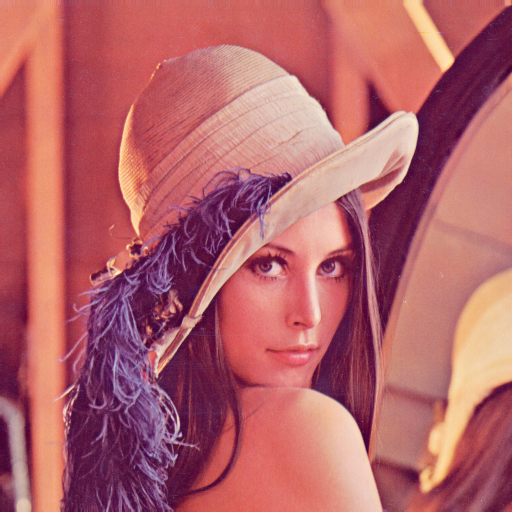
\includegraphics[width=0.5\textwidth]{imgs/lena.png}
	\caption{Ảnh mẫu Lena}
\end{figure}

\subsection{Điều chỉnh độ sáng}

\begin{figure}[H]
	\centering
	\subfloat[Tăng sáng (+40)]{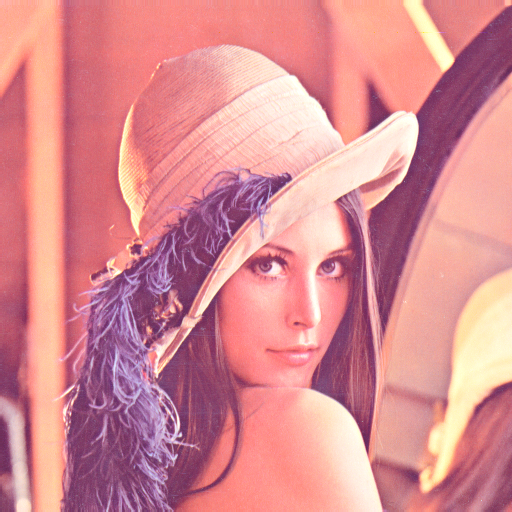
\includegraphics[width=0.45\textwidth]{imgs/lena_bright_up.png}}
	\hfill
	\subfloat[Giảm sáng (-40)]{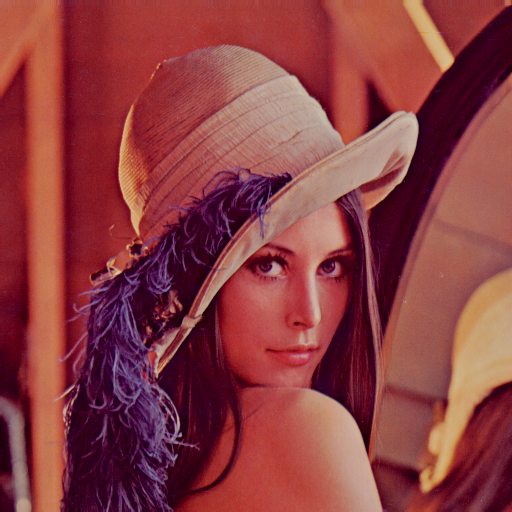
\includegraphics[width=0.45\textwidth]{imgs/lena_bright_down.png}}
	\caption{Ảnh sau khi điều chỉnh độ sáng}
\end{figure}

\subsection{Điều chỉnh độ tương phản}

\begin{figure}[H]
	\centering
	\subfloat[Tăng tương phản (1.5)]{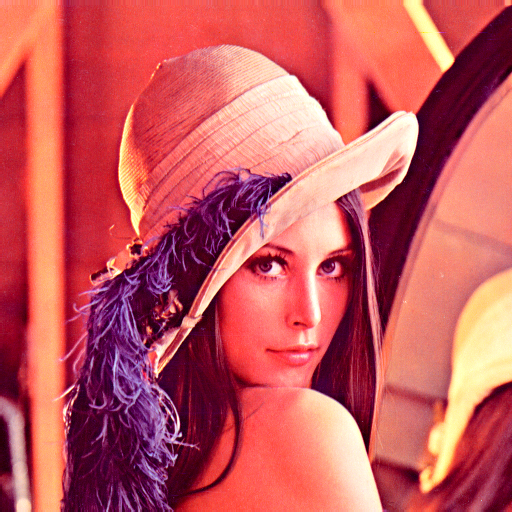
\includegraphics[width=0.45\textwidth]{imgs/lena_contrast_up.png}}
	\hfill
	\subfloat[Giảm tương phản (0.5)]{
\includegraphics[width=0.45\textwidth]{imgs/lena_contrast_down.png}}
	\caption{Ảnh sau khi điều chỉnh độ tương phản}
\end{figure}

\subsection{Lật ảnh}

\begin{figure}[H]
	\centering
	\subfloat[Lật ngang]{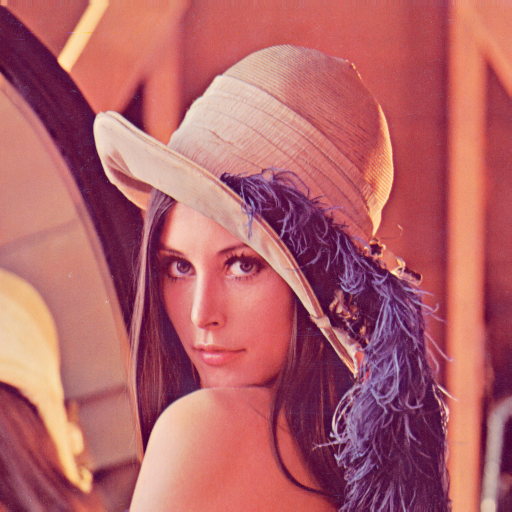
\includegraphics[width=0.45\textwidth]{imgs/lena_flip_horizontal.png}}
	\hfill
	\subfloat[Lật dọc]{
\includegraphics[width=0.45\textwidth]{imgs/lena_flip_vertical.png}}
	\caption{Kết quả lật ảnh}
\end{figure}

\subsection{Chuyển đổi màu sắc}

\begin{figure}[H]
	\centering
	\subfloat[Ảnh xám]{
\includegraphics[width=0.45\textwidth]{imgs/lena_gray.png}}
	\hfill
	\subfloat[Ảnh sepia]{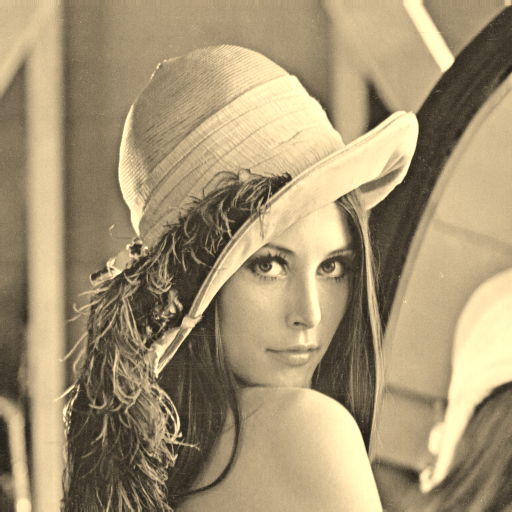
\includegraphics[width=0.45\textwidth]{imgs/lena_sepia.png}}
	\caption{Ảnh sau khi chuyển đổi màu sắc}
\end{figure}

\subsection{Làm mờ và sắc nét ảnh}

\begin{figure}[H]
	\centering
	\subfloat[Làm mờ (Blur)]{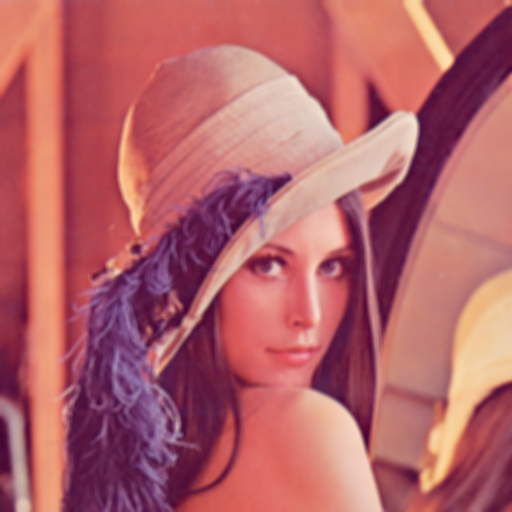
\includegraphics[width=0.45\textwidth]{imgs/lena_blur.png}}
	\hfill
	\subfloat[Làm sắc nét (Sharpen)]{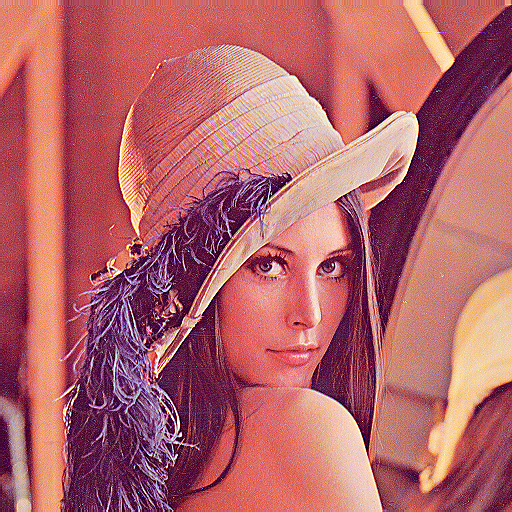
\includegraphics[width=0.45\textwidth]{imgs/lena_sharpen.png}}
	\caption{Ảnh sau khi áp dụng các bộ lọc}
\end{figure}

\subsection{Cắt ảnh theo khung hình vuông ở trung tâm}

\begin{figure}[H]
	\centering
	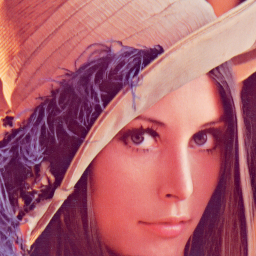
\includegraphics[width=0.5\textwidth]{imgs/lena_crop_center.png}
	\caption{Ảnh cắt ở trung tâm (size = \(256 \times 256\))}
\end{figure}

\subsection{Cắt ảnh theo khung hình tròn}

\begin{figure}[H]
	\centering
	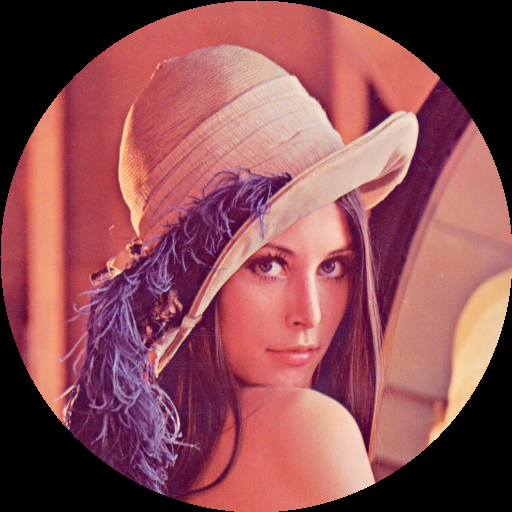
\includegraphics[width=0.5\textwidth]{imgs/lena_crop_circle.png}
	\caption{Ảnh cắt theo khung hình tròn}
\end{figure}

\subsection{Cắt ảnh theo khung hai hình ellipse chéo nhau}

\begin{figure}[H]
	\centering
	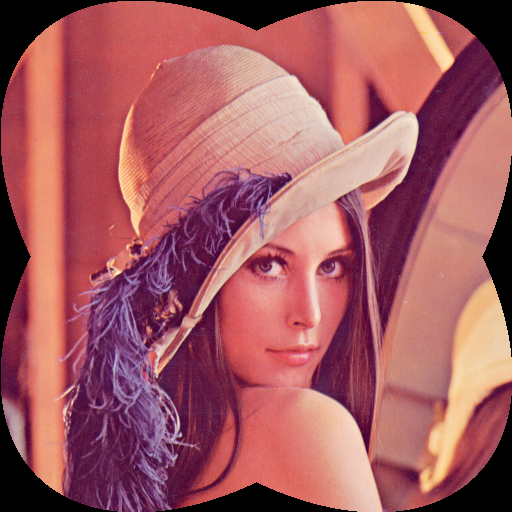
\includegraphics[width=0.5\textwidth]{imgs/lena_crop_ellipse.png}
	\caption{Ảnh cắt theo khung 2 hình ellipse chéo nhau (ratio = 0.6)}
\end{figure}

\subsection{Thời gian thực thi các chức năng}
\begin{table}[H]
	\centering
	\renewcommand{\arraystretch}{1.3}
	\caption{Thời gian thực thi của từng chức năng xử lý ảnh}
	\begin{tabular}{|p{10cm}|>{\raggedleft\arraybackslash}p{2cm}|}
		\hline
		\textbf{Chức năng}                            & \textbf{Thời gian} \\
		\hline
		Điều chỉnh độ sáng                            & 1.8ms              \\
		\hline
		Điều chỉnh tương phản                         & 4.4ms              \\
		\hline
		Lật ảnh ngang                                 & < 1ms              \\
		\hline
		Lật ảnh dọc                                   & < 1ms              \\
		\hline
		Chuyển ảnh RGB sang màu xám                   & 4.3ms              \\
		\hline
		Chuyển ảnh RGB sang màu sepia                 & 7.5ms              \\
		\hline
		Làm mờ ảnh                                    & 2760.7ms           \\
		\hline
		Làm sắc nét ảnh                               & 2635.1ms           \\
		\hline
		Cắt ảnh theo khung hình vuông ở trung tâm     & < 1ms              \\
		\hline
		Cắt ảnh theo khung hình tròn                  & 6.9ms              \\
		\hline
		Cắt ảnh theo khung hai hình ellipse chéo nhau & 15ms               \\
		\hline
	\end{tabular}
\end{table}


\newpage
\section{Acknowledgement}
Trong quá trình thực hiện báo cáo và xây dựng hệ thống xử lý ảnh, ChatGPT đã hỗ trợ sinh viên:

\begin{itemize}
	\item Đề xuất và soạn thảo template báo cáo LaTeX một cách rõ ràng và nhất quán.
	\item Viết \texttt{docstring} cho các hàm xử lý ảnh, giúp chuẩn hóa tài liệu và dễ dàng bảo trì mã nguồn.
	\item So sánh các loại kernel làm mờ phổ biến (Gaussian \(3\times3\), Gaussian \(5\times5\), Box Blur \(5\times5\), \ldots) và đề xuất lựa chọn kernel phù hợp giữa hiệu quả làm mờ và độ phức tạp tính toán.
	\item Đề xuất ý tưởng và chứng minh công thức tính hai bán kính của elip cho tính năng cắt ảnh theo khung 2 hình elip chéo nhau (\texttt{double\_ellipse\_crop}).
	\item Hỗ trợ viết hàm đo thời gian thực thi (\texttt{benchmark}) cho từng hàm xử lý ảnh, giúp đánh giá hiệu suất và tối ưu hóa.
\end{itemize}


\begin{thebibliography}{9}

  \bibitem{wikipedia_kernel}
  Wikipedia, 
  \textit{Kernel (image processing)}, truy cập ngày 22/07/2025,
  \newline
  \url{https://en.wikipedia.org/wiki/Kernel_(image_processing)}

  \bibitem{dyclassroom_sepia}
  dyclassroom.com, 
  \textit{How to convert a color image into sepia image}, truy cập ngày 20/07/2025,
  \newline
  \url{https://dyclassroom.com/image-processing-project/how-to-convert-a-color-image-into-sepia-image}

  \bibitem{matlab_rgb2gray}
  MathWorks, 
  \textit{Convert RGB image or colormap to grayscale}, truy cập ngày 20/07/2025,
  \newline
  \url{https://www.mathworks.com/help/matlab/ref/rgb2gray.html}

  \bibitem{gonzalez_woods}
  Gonzalez, R. C. \& Woods, R. E., 
  \textit{Digital Image Processing}, 4th Edition, Chương 3: Intensity Transformations and Spatial Filtering, truy cập ngày 18/07/2025,
  \newline
  \url{https://www.cl72.org/090imagePLib/books/Gonzales,Woods-Digital.Image.Processing.4th.Edition.pdf}

\end{thebibliography}



\pagebreak
\end{document}